\documentclass[11pt,a4paper]{article}
\usepackage[T1]{fontenc}
\usepackage[utf8]{inputenc}
\usepackage[margin=1in]{geometry}
\usepackage{graphicx}
\usepackage{float}
\usepackage[hidelinks]{hyperref}

\title{Supplementary Diagnostic Figures\\
Commodity Tail Dependence and Exchange-Rate Risk in Ghana}
\author{Jonathan Nelson\\Kwame Nkrumah University of Science and Technology (KNUST), Kumasi, Ghana}
\date{}

\begin{document}
\maketitle

\setcounter{figure}{0}
\renewcommand{\thefigure}{S\arabic{figure}}

\begin{figure}[H]
\centering
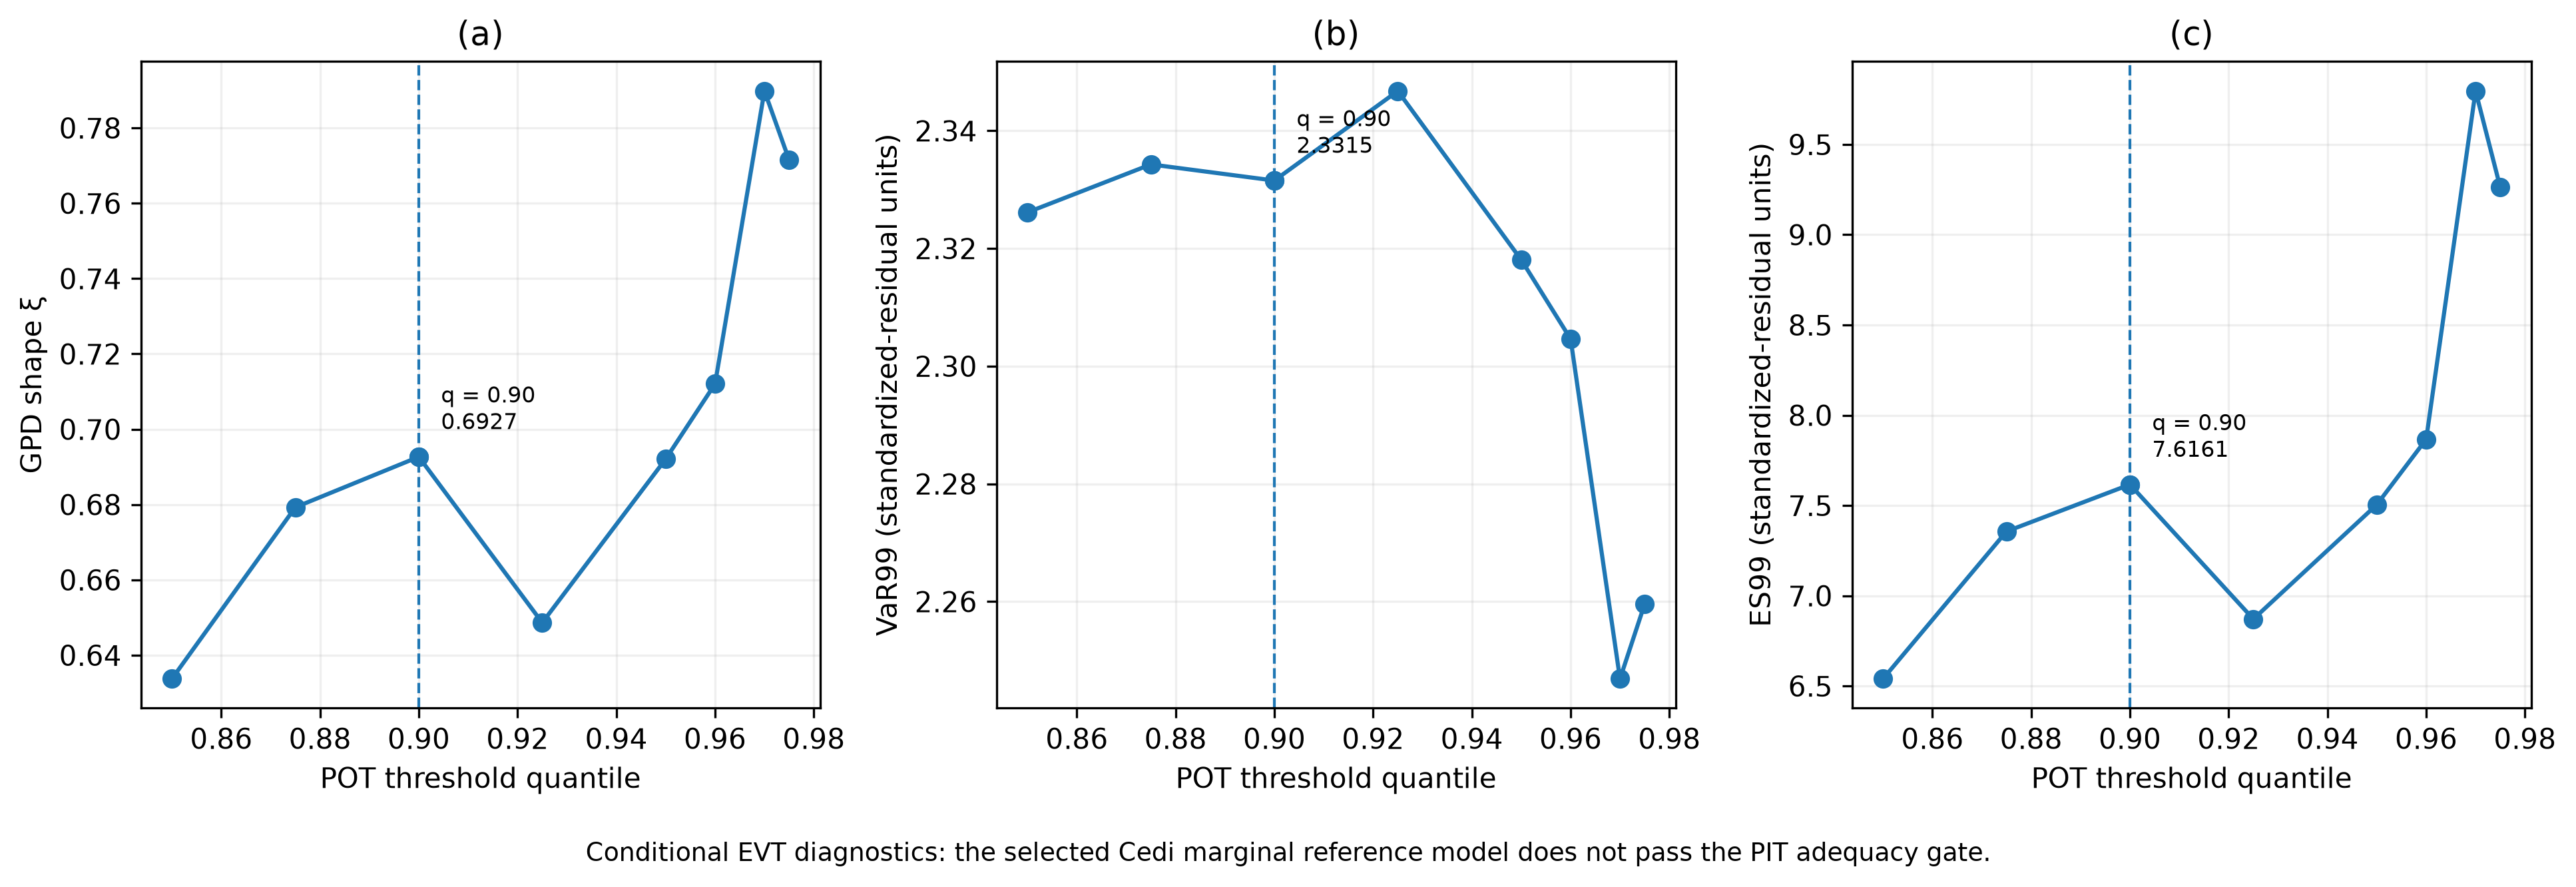
\includegraphics[width=0.96\linewidth]{figures/figure_S1_cedi_evt_threshold_sensitivity.png}
\caption{Panel B Cedi EVT threshold sensitivity. The estimates are conditional diagnostics because the selected Cedi marginal reference model is inadequate.}
\label{fig:s1-evt}
\end{figure}

\clearpage

\begin{figure}[H]
\centering
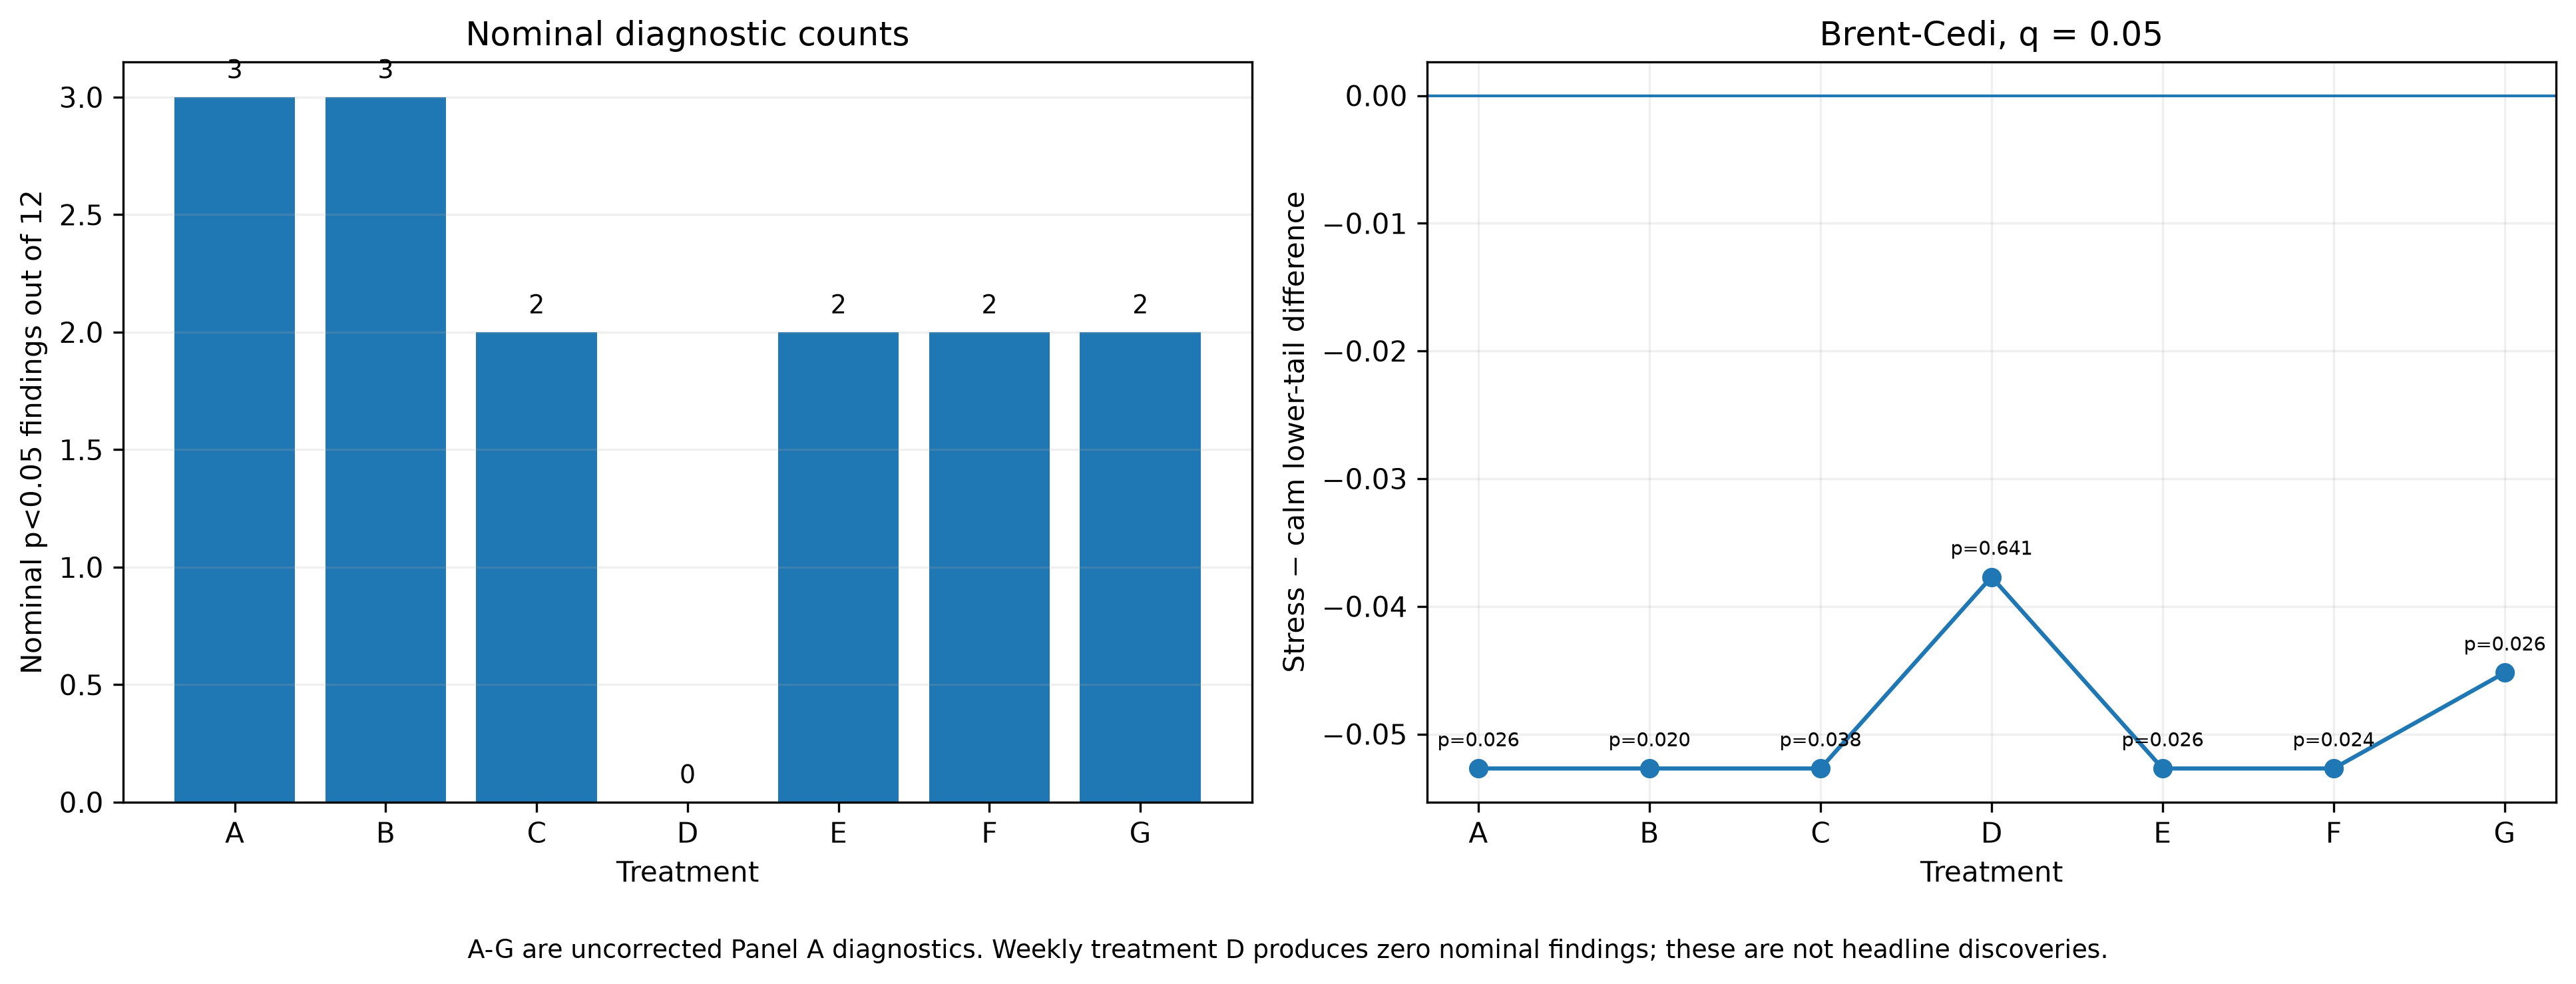
\includegraphics[width=0.96\linewidth]{figures/figure_S2_cedi_AG_sensitivity.png}
\caption{Panel A Cedi A--G sensitivity diagnostics. The displayed counts and $p$-values are uncorrected diagnostics and are not treated as headline discoveries.}
\label{fig:s2-ag}
\end{figure}

\clearpage

\begin{figure}[H]
\centering
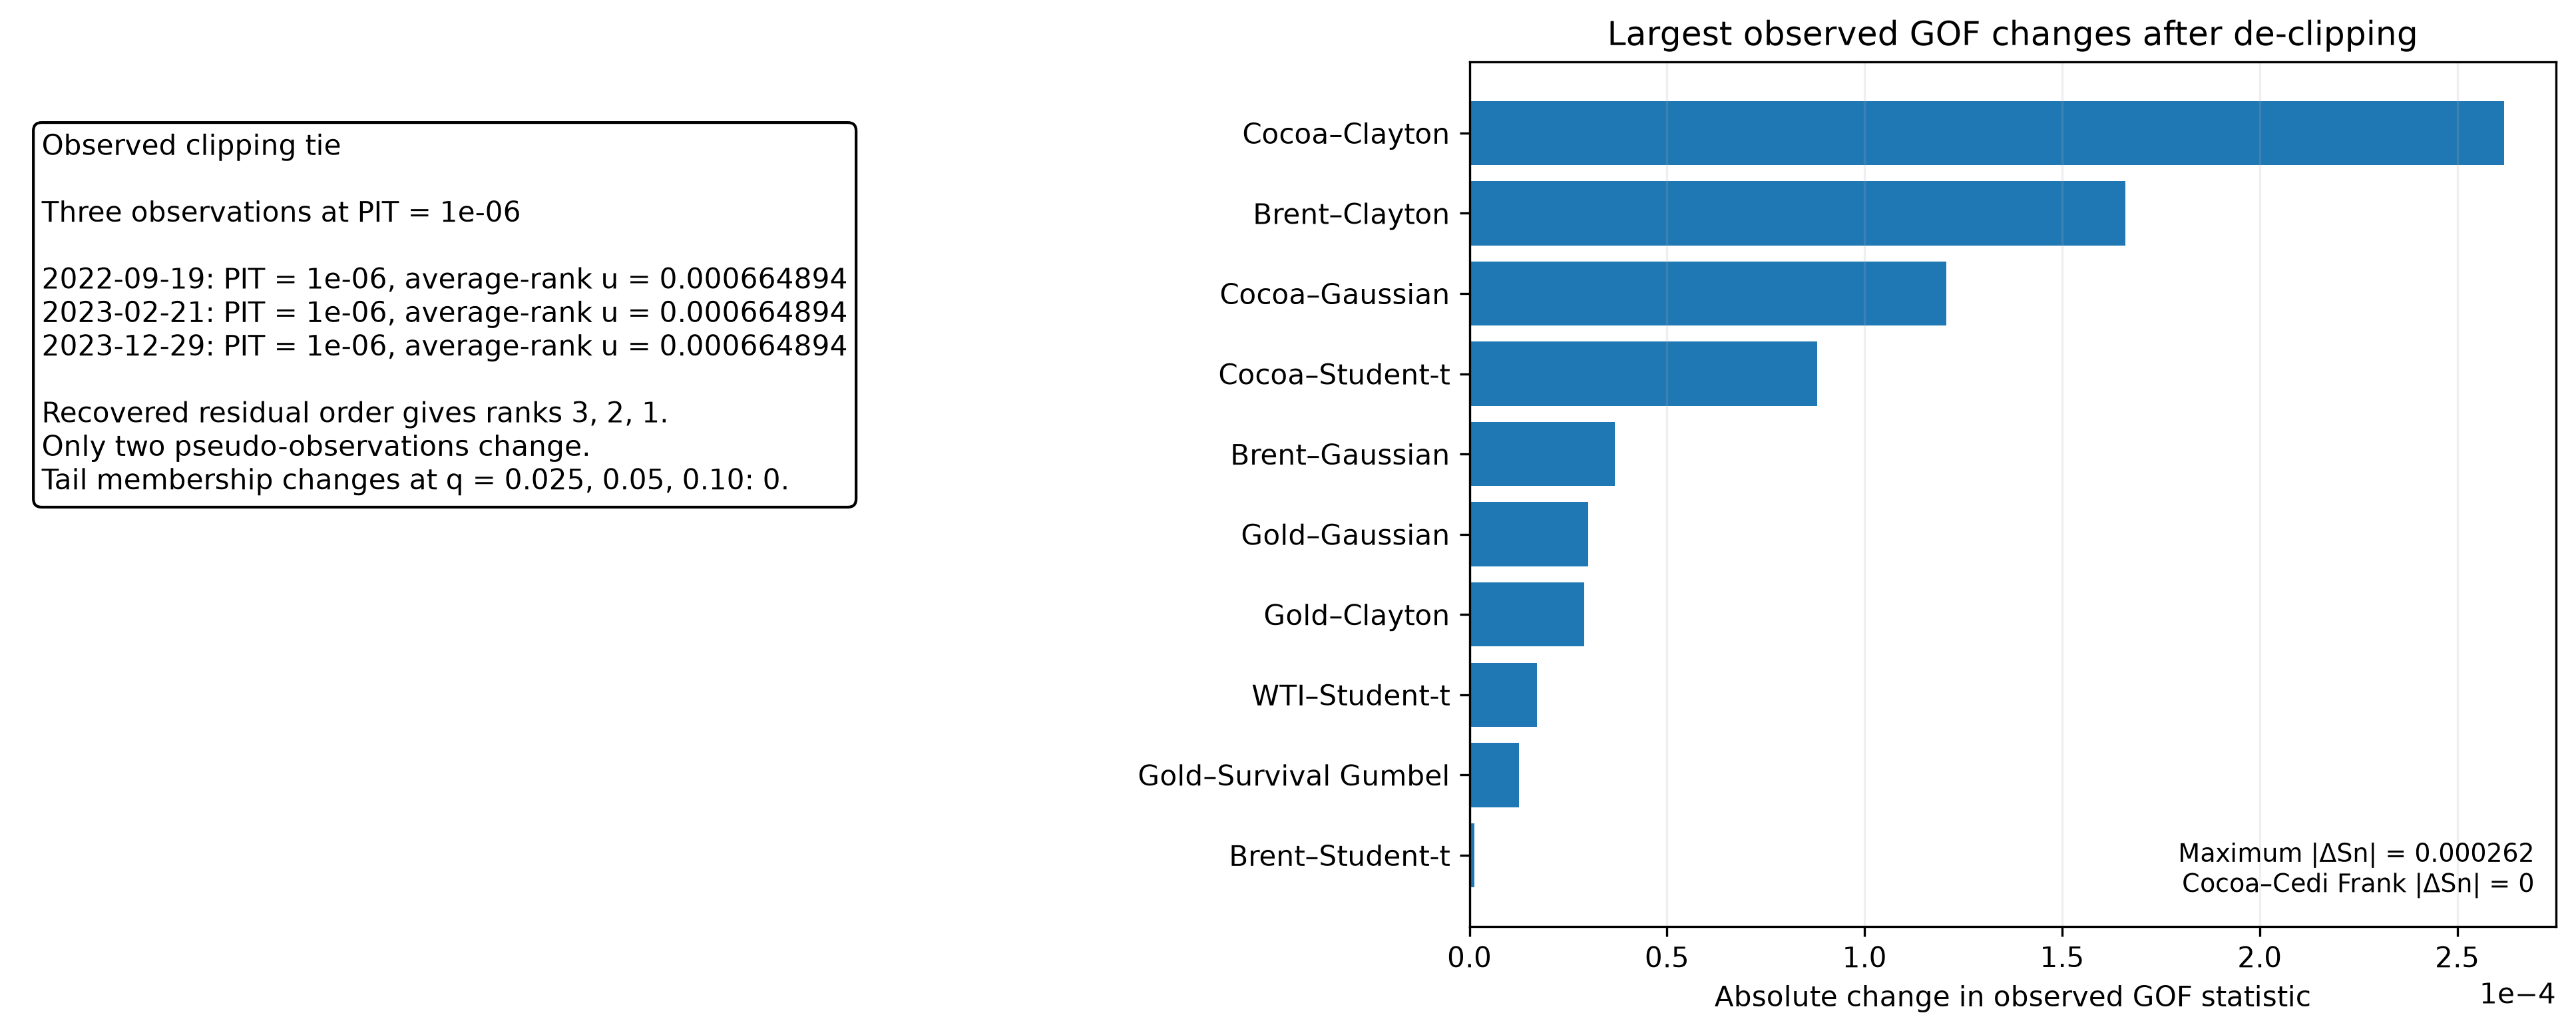
\includegraphics[width=0.96\linewidth]{figures/figure_S3_pit_clipping_diagnostic.png}
\caption{Panel A Cedi PIT-clipping diagnostic. The clipping tie has negligible numerical consequences for the prespecified tail sets and observed copula goodness-of-fit statistics.}
\label{fig:s3-pit}
\end{figure}

\end{document}
